\subsection{Hydrogen Cryotarget}\label{sec:clas.tgt}


The target used by \g12 was conical as shown in Fig.~\ref{fig:clas.targetblueprint}. The target walls were constructed of 0.127~$\mu$m thick Kapton. It is 40~cm in length and 2~cm in radius. The incident photon beam had a radius of 1.5~cm. The target cell design shown in Figs,~\ref{fig:clas.targetblueprint} and~\ref{fig:clas.targetcell} had been used in several experiments and is capable of containing a number of different materials, such as helium, deuterium and hydrogen. For \g12 the target was filled with liquid hydrogen ($\ell$H$_2$). The temperature and pressure of the target was continuously measured and recorded. In Sec~\ref{sec:analysis.target_density}, these measurements will be used to calculate the density of the liquid Hydrogen to determine the target thickness. The target was not polarized.

\begin{figure}[h!]\begin{center}
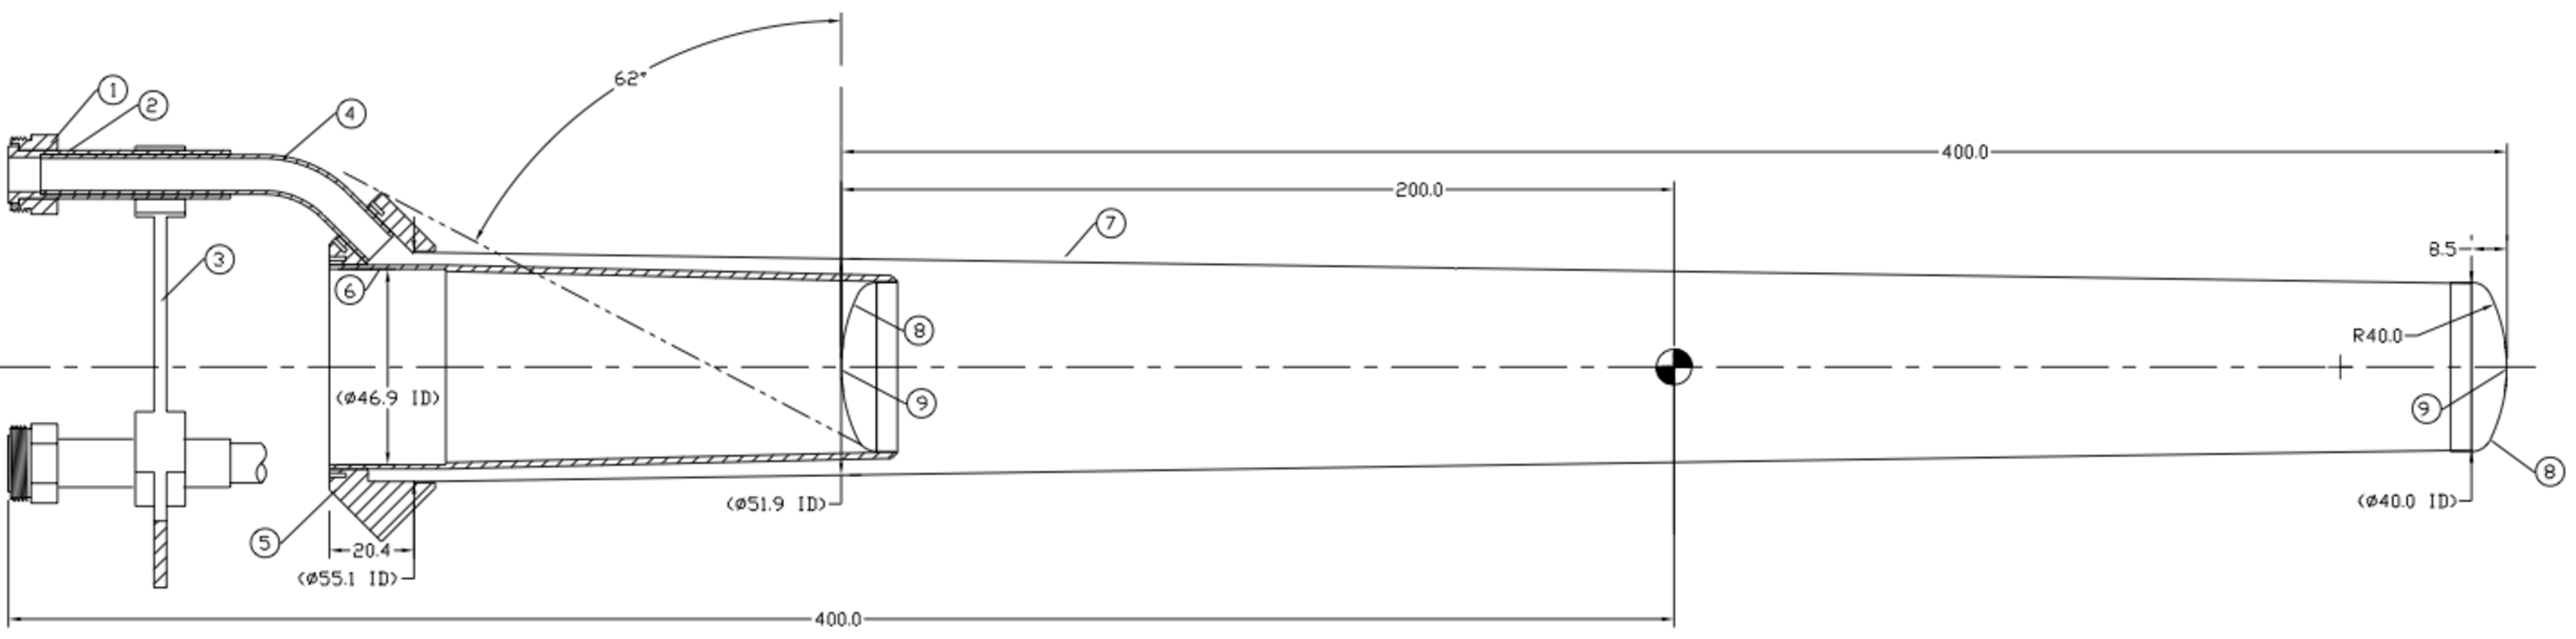
\includegraphics[width=\figwidth,height = \qfigheight]{\grpath/hall-b/g11_target_cell_blueprint.pdf}
\caption[Blueprint schematic of the conical Kapton target cell used for \g12]{\label{fig:clas.targetblueprint}Blueprint schematic of the conical Kapton target cell used for \g12.}
\end{center}\end{figure}

\begin{figure}[h!]\begin{center}
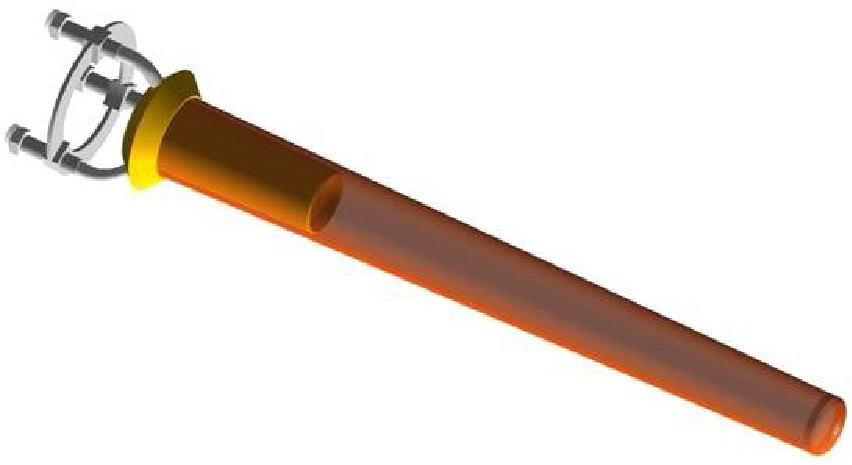
\includegraphics[width=0.6\figwidth]{\grpath/hall-b/g11_target_cell.pdf}
\caption[The 40~cm long conical Kapton target cell used for \g12]{\label{fig:clas.targetcell}The 40~cm long conical Kapton target cell used for \g12.}
\end{center}\end{figure}

%\subsubsection{Target Position for \g12}\label{sec:clas.tgt.position}
The target was located 90~cm upstream of \abbr{CLAS} the center, see Fig.~\ref{fig:clas.ced}.
This increased the forward angle acceptance from 8$^\circ$  to 6$^\circ$. However, this also decreased the large angle acceptance from approximately 140$^\circ$ to 100$^\circ$ in the lab frame.
%This reduction in large angle acceptance sacrificed multi-particle final state events, where the final state particles were more than about 70$^\circ$ away from beamline.
%as well as a reduction in \abbr{DC} resolution. The \abbr{DC} resolution decrease was due to the oblique angle the tracks made with the detector planes.
\FloatBarrier